\documentclass[oneside]{article}

% Package necessari
\usepackage[a4paper,top=2cm,bottom=2cm,left=1.5cm,right=1.5cm]{geometry}
\usepackage[utf8]{inputenc}
\usepackage[italian]{babel}
\usepackage[T1]{fontenc}
\usepackage{amsmath}
\usepackage{amssymb}
\usepackage{graphicx}
\usepackage[table, dvipsnames]{xcolor}
\usepackage{listings}
\usepackage{hyperref}
\usepackage{enumitem}
\usepackage{fancyhdr}
\usepackage{cancel}
\usepackage[ruled,vlined,linesnumbered]{algorithm2e}
\usepackage[noend]{algpseudocode}
\usepackage[font={small,sl}]{caption}
\usepackage[font={small,sl}]{subcaption}
\usepackage{tocbibind}
\usepackage{accents}
\usepackage[section]{placeins}
\usepackage{multicol}
\usepackage{mathtools}
\usepackage{dsfont}
\usepackage{color}
\usepackage{titlesec}

\makeatletter
\AtBeginDocument{%
  \expandafter\renewcommand\expandafter\subsection\expandafter{%
    \expandafter\@fb@secFB\subsection
  }%
}
\makeatother

% Colori per i listing
\definecolor{code_red}{rgb}{0.6,0,0} % strings
\definecolor{code_green}{rgb}{0.25,0.5,0.35} % comments
\definecolor{code_purple}{rgb}{0.5,0,0.35} % keywords
\definecolor{code_background}{rgb}{0.95,0.95,0.92} % background
\definecolor{verify_blue}{HTML}{12ACF2}
\definecolor{verify_red}{HTML}{F2122C}
\definecolor{verify_yellow}{HTML}{FFBB00}

% Stile del codice standard (C)
\lstset{
	language=C, 
	backgroundcolor=\color{code_background},
	frame=single,
	basicstyle=\ttfamily\small,
	keywordstyle=\color{code_purple}\bfseries\small,
	stringstyle=\color{code_red}\small,
	commentstyle=\color{code_green}\small,
	numbers=left,
	numberstyle=\small\color{gray},
	numbersep=5pt,
	tabsize=4,
	showtabs=false,
	showspaces=false,
	showstringspaces=false,
	escapechar=|, 
	captionpos=b,
	breaklines=true,
}

% Aggiunto paragraph come subsubsubsection
\setcounter{secnumdepth}{3}
\titleformat{\paragraph}
{\normalfont\normalsize\bfseries}{\theparagraph}{1em}{}
\titlespacing*{\paragraph}
{0pt}{3.25ex plus 1ex minus .2ex}{1.5ex plus .2ex}

% Impostazione delle lunghezze di alcuni elementi del documento
\setlength{\parskip}{1em}
\setlength{\parindent}{0em}
\setlength{\arrayrulewidth}{0.1em}

% Informazioni per la title page
\title{Progetto di Sistemi Operativi Avanzati}

\date{A.A. 2021/2022}

\author{A. Chillotti\thanks{\texttt{\href{mailto:alessandro.chillotti@outlook.it}{alessandro.chillotti@outlook.it}}}}

% Impostazione del package hyperref
\hypersetup{
    colorlinks=true,
    linktocpage=true,
    linkcolor=blue,
    urlcolor=blue,
    pdftitle={Advanced Operating Systems and System Security},
    pdfauthor={A. Chillotti},
}
 
% Stile del codice standard (C)
\lstset{
	language=C, 
	backgroundcolor=\color{code_background},
	frame=single,
	basicstyle=\ttfamily\small,
	keywordstyle=\color{code_purple}\bfseries\small,
	stringstyle=\color{code_red}\small,
	commentstyle=\color{code_green}\small,
	numbers=left,
	numberstyle=\small\color{gray},
	numbersep=5pt,
	tabsize=4,
	showtabs=false,
	showspaces=false,
	showstringspaces=false,
	escapechar=|, 
	captionpos=b,
	breaklines=true,
}

\pagestyle{fancy}
\fancyhf{}
\lhead{\small A.Chillotti}
\rhead{\small Advanced Operating Systems and System Security}
\cfoot{\thepage}
%\cfoot{Pagina \thepage}
\SetNlSty{bfseries}{\color{black}}{}

% Spaziatura tabelle
\renewcommand{\arraystretch}{1.5}

\graphicspath{ {./figs/} }
% Definizione del colore delle tabelle
\newcommand{\tablecolors}[1][2]{\rowcolors{#1}{yellow!50}{yellow!25}}

% Definizione dello stile da usare per la P di probabilità (grassetto in math-mode)
\newcommand{\pr}{\mathbf{P}}

% Forzatura del displaystyle in math-mode
\everymath\expandafter{\the\everymath\displaystyle}

%\newcommand{\scaption}[1]{\small{\caption{#1}}}
\renewcommand{\lstlistingname}{Snippet}

% Definizione di comandi per operatori matematici
\newcommand{\xor}{\oplus}

% Definizione osservazione
\newcommand{\obs}{\underline{Osservazione}}

% Definizione di \texttt{•} per matematica
\newcommand{\matht}[1]{\text{\texttt{#1}}}

% Definizione di domande e risposta
\newcommand{\question}[2]{
\textit{#1}\\
#2
}

\begin{document}
\maketitle

\section{Traccia del progetto (traduzione)}
Questa specifica è legata ad un driver Linux che implementa flussi di dati a priorità bassa e alta. Attraverso una sessione aperta al devide file, un thread può leggere/scrivere segmenti dati. La consegna dei dati segue una policy First-in-First-out lungo ciascuno dei due diversi flussi di dati (bassa e alta priorità). Dopo le operazioni di lettura, i dati devono scomparire dal flusso. Inoltre, il flusso dati di alta priorità deve offrire operazioni di scrittura sincrone, mentre il flusso dati di bassa priorità deve offrire una esecuzione asincrona (basata su delayed work) delle operazioni di scrittura, pur mantenendo l'interfaccia in grado di notificare in modo sincrono l'esito. Le operazioni di lettura sono tutte eseguite sincronamente. Il device driver supporta 128 device corrispondenti alla stessa quantità di minor number. Il device driver deve implementare il supporto per il servizio \texttt{ioctl(..)} in modo tale da gestire la sessione di I/O come segue:
\begin{itemize}
\item setup del livello di priorità (alto o basso) per le operazioni;
\item operazioni di lettura e scrittura bloccanti vs operazioni di lettura e scrittura non bloccanti;
\item setup del timeout che reluga il risveglio delle operazioni bloccanti.
\end{itemize}
Alcuni parametri e funzioni del modulo Linux dovrebbero essere in grado di abilitare o disabilitare il file del dispositivo, in termini di specifico minor number. Se è disabilitato, un tentativo di apertura della sessione deve fallire (ma le sessioni già aperte devono essere ancora gestire). Ulteriori parametri esposti via VFS devono fornire un'immagine dello stato corrente del device in accordo alle seguenti informazioni:
\begin{itemize}
\item abilitiato o disabilitato;
\item numero di byte correntemente presente nei due flussi (alta e bassa priorità);
\item numero di thread correntemente in attesa di dati lungo i due flussi (alta e bassa priorità).
\end{itemize}

\section{Relazione del progetto svolto}
\subsection{Rappresentazione dei multi-flow device file}
La rappresentazione dei multi-flow device file è definita dalla struttura \texttt{object\_t} che contiene:
\begin{itemize}
\item un puntatore ad una workqueue, ovvero \texttt{struct workqueue\_struct *workqueue}. Il puntatore alla workqueue è stato inserito all'interno della struttura rappresenta il multi-flow device file perché è utile solo nel caso in cui si sta lavorando a \texttt{LOW PRIORITY}.
\item due puntatori ad un buffer, ovvero \texttt{dynamic\_buffer\_t *buffer}.
\end{itemize}

\subsection{Rappresentazione del buffer}
La rappresentazione del buffer è definita dalla struttura \texttt{dynamic\_buffer} che contiene:
\begin{itemize}
\item un puntatore \texttt{head} di tipo \texttt{data\_segment};
\item un puntatore \texttt{tail} di tipo \texttt{data\_segment};
\item un mutex che permette di sincronizzare le operazioni relative al buffer;
\item una waitqueue.
\end{itemize}

L'organizzazione della rappresentazione del buffer è rappresentata dalla seguente figura.

\begin{figure}[ht!]
\centering
\frame{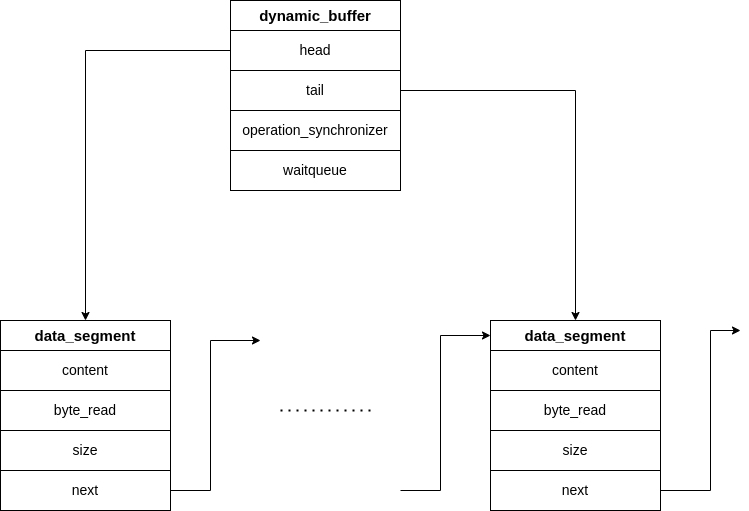
\includegraphics[width=0.5\textwidth]{img/data-segment}}
\end{figure}

Si può notare come siamo presenti \texttt{256} waitqueue, ovvero una per ogni buffer. Questa scelta è stata fatta perché il lavoro svolto su un altro buffer è sicuramente indipendente dal lavoro fatto da un altor buffer. Inoltre, nella funzione di inizializzazione del modulo vengono create delle singlethread workqueue. In questo modo il deferred work viene processato lungo un unico kworker deamon ed esso riporta le operazioni di scrittura sul buffer di bassa priorità nel medesimo ordine con cui sono state schedulate, senza dover implementare meccanismi di ordinamento e sincronizzazione.

\subsection{Parametri del modulo}
Sono stati definiti dei parametri del modulo ed essi sono stati utilizzati all'interno del driver come variabili operative. In particolare sono stati definiti i seguenti parametri:
\begin{itemize}
\item \texttt{enabled}: un vettore di \texttt{128} elementi di tipo \texttt{bool}, ove ogni elemento \texttt{i} indica se il multi-flow device file relativo al minor number \texttt{i} è attivo o meno;
\item \texttt{byte\_in\_buffer}: un vettore di \texttt{256} elementi di tipo \texttt{long}, ove ogni elemento riporta il numero di byte presente all'interno del buffer relativo ad uno specifico minor number, in particolare:
\begin{itemize}
\item i primi \texttt{128} elementi sono relativi al buffer di bassa priorità del multi-flow device file con minor number \texttt{i};
\item i secondi \texttt{128} elementi sono relativi al buffer di alta priorità del multi-flow device file con minor number $\frac{\mathtt{i}}{\mathtt{2}}$;
\end{itemize}
\item \texttt{thread\_in\_wait}: un vettore di \texttt{256} elementi di tipo \texttt{long}, ove ogni elemento riporta il numero di byte presente all'interno del buffer relativo ad uno specifico minor number, secondo la medesima regola di \texttt{byte\_in\_buffer}.
\end{itemize}

La scelta di creare un vettore di \texttt{256} elementi anziché \texttt{128} è stata fatta perché ha permesso la realizzazione di un codice migliore dal punto di vista della leggibilità. Questo perché, indipendemente dalla priorità, prima di andare ad effettuare una scrittura o una lettura si effettua un controllo sul contento del buffer (i.e. spazio libero in caso di scrittura, byte nel buffer in caso di scrittura). Infatti, nel caso in cui si fossero creati due vettori da \texttt{128} elementi si sarebbero dovuti differenziare i casi. A tal proposito è stata realizzata la seguente macro:
\begin{lstlisting}
#define get_byte_in_buffer_index(priority, minor)	\
        ((priority * MINOR_NUMBER) + minor)
\end{lstlisting}

\subsection{Operazioni sui multi-flow device file}
Nelle seguenti sottosezioni sono descritte le funzioni che compongono il driver.

\subsection{Operazione d'apertura}
La funzione \texttt{dev\_open} consente l'apertura 

\subsection{Operazione di rilascio}
\subsection{Operazione di scrittura}
\subsection{Operazione di lettura}


\end{document}
